\subtitlepage{SaltStack}{Начало}

\begin{Frame}{SaltStack --- это}
  \begin{itemize}[<+-| alert@ +>]
    \item[\faWrench] Система управления конфигурациями\\
    \item[{\faCircle[regular]}] Шина на ZeroMQ\footnote<.->{\url{https://zeromq.org/}}
    \item[\faCubes] Python и модульность
    \item[\faIndent] Профессия YAML-программист
    \item[\faCloud] \relax <<Провиженинг>> для IaaS
    \item[\faCube] В народе --- <<соль>>
  \end{itemize}

  \vfill

  \begin{center}
    
\includegraphics[width=240pt]{saltstack-logo}
  \end{center}

\end{Frame}

\begin{Frame}{Системы управления конфигурациями}

  \setbeamercovered{invisible}

  \centering
  \def\arraystretch{1.5}
  \begin{table}\begin{tabularx}{\textwidth}{r|lp{6em}p{4em}X}
    СУК & Год & На чём & DSL & Особенности \\
    \hline
    \onslide<+->{
      \alert<.>{Puppet} & 2005 & Ruby & Свой & Pull \\
    }
    \onslide<+->{
      \alert<.>{Chef} & 2009 & Ruby, Erlang & Ruby & Pull, веб-интерфейс} \\
    \onslide<+->{
      \alert<.>{\bf SaltStack} & \bf 2011 &
      \bf Python\footnote{Сплошной Python} & \bf YAML & \bf Pull (и Push),
      корп-версия\\
    }
    \onslide<+->{
      \alert<.>{Ansible} & 2012 & Python, Ruby & YAML &
      Push (и Pull), Ansible Tower
    }
  \end{tabularx}\end{table}
\end{Frame}

\liveframe{}

\begin{Frame}{Глоссарий}
  \centering
  \def\arraystretch{1.5}
  \small
  \begin{table}\begin{tabularx}{\textwidth}{l|X|l}
    В SaltStack & Значение & В Ansible \\
    \hline
    Мастер & Сервер & Узел (нода) управления \\
    Миньон & Клиент & Управляемый узел \\
    Формула & Декларативный конфиг клиента & Плейбук\\
    Состояние & Элементарная единица конфига клиента & Таск \\
    Грейн & Переменная, полученная от клиента & Факт \\
    Топ-файл & Маппинг хостов & Инвентарь (хосты)\\
    Пиллары & Устанавливаемая переменная & Инвентарь (переменные) \\
  \end{tabularx}\end{table}
\end{Frame}

\begin{Frame}{Топология}
  \centering
  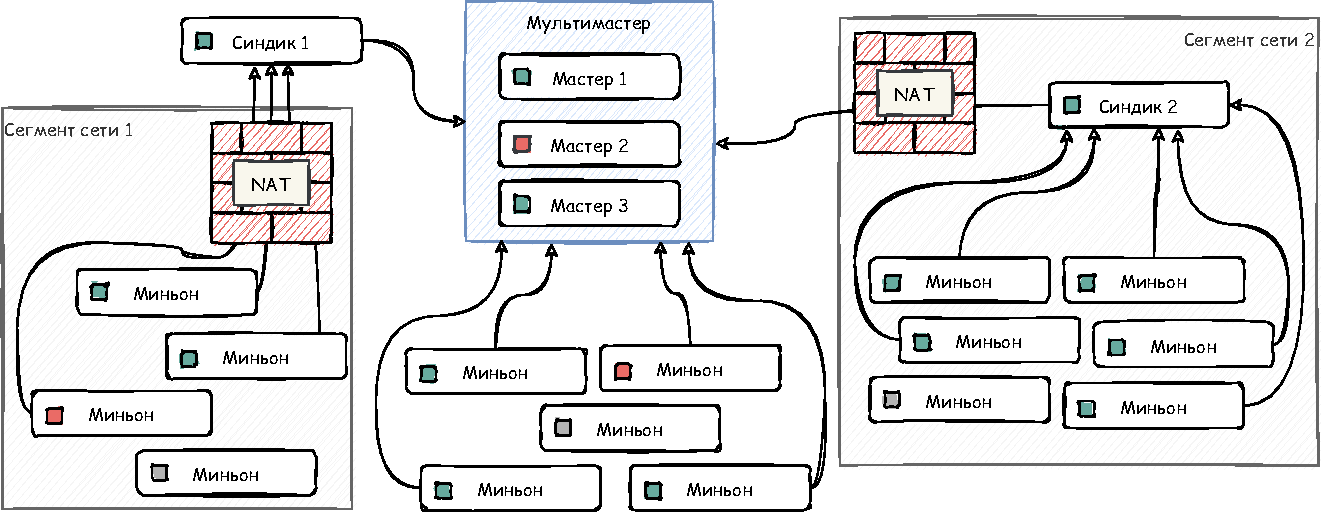
\includegraphics[width=0.95\textwidth]{saltstack-topology}
\end{Frame}

\begin{Frame}{Архитектура}
  \centering
  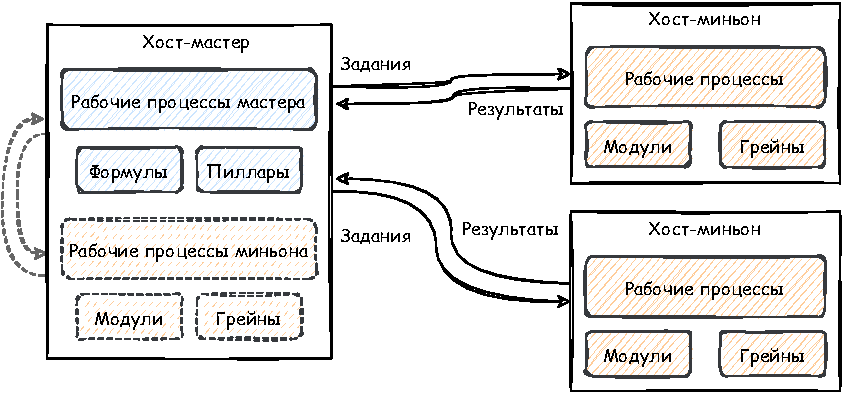
\includegraphics[width=0.80\textwidth]{saltstack-architecture}
\end{Frame}

\begin{Frame}{Данные}
  \begin{columns}
    \begin{column}{0.45\textwidth}
      \begin{itemize}[<+-| alert@ +>]
        \item Grains (<<крупицы соли>>) \baselinespace
        \item Pillars (<<соляные столпы>>) \baselinespace
        \item Salt Mine (<<соляная шахта>>)
      \end{itemize}
    \end{column}
    \begin{column}{0.55\textwidth}
      \includegraphics<1>[width=0.9\textwidth]{grains-photo}
      \includegraphics<2>[width=0.9\textwidth]{salt-pillar}
      \includegraphics<3>[width=0.9\textwidth]{salt-mine-photo}
    \end{column}
  \end{columns}
\end{Frame}

\begin{Frame}{Типы модулей}
  \overlaypic{south east}{width=100pt}{boxes}
  \begin{itemize}[<+-| alert@ +>]
    \item \texttt{salt.modules}
    \item \texttt{salt.states}
    \item \texttt{salt.grains}
    \item \texttt{salt.pillar}
    \item \texttt{salt.renderer}
    \item \ldots
    \item Десятки их!
  \end{itemize}
\end{Frame}

\begin{Frame}{YAML}
  \centering
  \huge У вас найдётся минутка поговорить о ещё одном языке разметки?
\end{Frame}

\begin{frame}{YAML}
  \ExampleNote{}

  \begin{columns}
    \begin{column}{0.5\textwidth}
      \begin{itemize}[<+-| alert@ +>]
        \item Форматирование отступами
        \item Скалярные типы
        \item Мультистрочные литералы\footnotemark{}
        \item Словари и последовательности
        \item Включает в себя JSON
        \item Наследование (на десерт)
      \end{itemize}
    \end{column}

    \begin{column}{0.5\textwidth}
      \inputminted{yaml}{../examples/yaml-file.yaml}
    \end{column}
  \end{columns}

  \onslide<3->\footnotetext{\url{https://yaml-multiline.info}}

\end{frame}
